\documentclass[10pt]{beamer}

\usetheme{metropolis}
\usepackage{appendixnumberbeamer}

\usepackage{booktabs}
\usepackage[scale=2]{ccicons}

\usepackage{pgfplots}
\usepgfplotslibrary{dateplot}

\usepackage{xspace}
\newcommand{\themename}{\textbf{\textsc{metropolis}}\xspace}

\title{Understanding the PhD Landscape in Europe and Germany}
\subtitle{Talk 1: Preparing for and Starting Your PhD Journey}
\date{\today}
\author{Dr. Bijun Li}
%\institute{Center for modern beamer themes}
% \titlegraphic{\hfill\includegraphics[height=1.5cm]{logo.pdf}}

\begin{document}

\maketitle

%\section{Introduction}

% new page 
\begin{frame}[fragile]{Self-Introduction}
\begin{itemize}
    \item Dr. Bijun Li
    \item PhD in Computer Science from [University Name]
    \item Research focus: [Brief description of research area]
    \item Current position: [e.g., Postdoctoral Researcher at XYZ University]
    \item Experience with international academic environments
    \item Passionate about guiding students in their academic journey
\end{itemize}
\end{frame}

% new page
\begin{frame}[fragile]{Purpose of the Series}
\begin{columns}[T]
    \begin{column}{0.6\textwidth}
        \alert{Explore PhD Opportunities in Europe}
        \begin{itemize}
            \item Comprehensive overview of European PhD landscape
            \item In-depth focus on Germany's prestigious programs
            \item Detailed guidance on application process
            \item Insights into funding and practical considerations
        \end{itemize}
    \end{column}
    \begin{column}{0.4\textwidth}
        \alert{Target Audience}
        \begin{itemize}
            \item Current Master's students
            \item Final-year undergraduates
            \item Early-career professionals considering academia
        \end{itemize}
        % Add an icon or image representing diverse students
        %\includegraphics[width=\textwidth]{diverse_students_icon.png}
    \end{column}
\end{columns}
\end{frame}

% new page
\begin{frame}[fragile]{Overview of Talk 1}
\begin{columns}[T]
    \begin{column}{0.5\textwidth}
        \alert{1. PhD Programs in Europe}
        \begin{itemize}
            \item General structure and duration
            \item Comparative analysis across countries
        \end{itemize}
        \alert{2. German Higher Education System}
        \begin{itemize}
            \item Types of institutions
            \item Research and industry collaborations
        \end{itemize}
    \end{column}
    \begin{column}{0.5\textwidth}
        \alert{3. Finding PhD Opportunities}
        \begin{itemize}
            \item Research methods and resources
            \item Contacting potential supervisors
            \item Networking strategies
        \end{itemize}
        \alert{4. Application Process}
        \begin{itemize}
            \item Eligibility criteria
            \item Required documents
            \item Application timeline
        \end{itemize}
    \end{column}
\end{columns}
\end{frame}

% new page
\begin{frame}[fragile]{PhD Programs in Europe: Comparative Analysis}
\begin{tabular}{|l|c|c|c|c|}
\hline
\textbf{Aspect} & \textbf{Germany} & \textbf{France} & \textbf{Netherlands} & \textbf{Scandinavia} \\
\hline
Duration & 3-5 years & 3-4 years & 4 years & 3-4 years \\
\hline
Structure & Research-focused & Coursework + Research & Structured & Project-based \\
\hline
Funding & Often employed & Varied & Employed & Employed \\
\hline
Teaching & Optional & Limited & Often required & Often required \\
\hline
Industry links & Strong & Moderate & Strong & Strong \\
\hline
\end{tabular}

\vspace{0.5cm}
\alert{Key Differences}
\begin{itemize}
    \item Germany: Strong industry collaborations, research-intensive
    \item France: More structured programs, linked to research institutions
    \item Netherlands: Clear timelines, teaching responsibilities
    \item Scandinavia: Focus on societal impact, public engagement
\end{itemize}
\end{frame}

% new page
\begin{frame}[fragile]{Overview of the German Higher Education System}
    \begin{columns}[T]
        \begin{column}{0.5\textwidth}
            \textbf{Research Universities (Universitäten)}
            \begin{itemize}
                \item Focus: Academic research, theoretical knowledge
                \item Strengths: Extensive research, doctoral programs
                \item Examples: 
                    \begin{itemize}
                        \item TU Munich
                        \item Heidelberg University
                        \item University of Freiburg
                    \end{itemize}
            \end{itemize}
            
            \vspace{0.5cm}
            
            \textbf{Universities of Applied Sciences}
            \begin{itemize}
                \item Focus: Practice-oriented, applied research
                \item Strengths: Industry ties, practical skills
                \item Examples:
                    \begin{itemize}
                        \item Munich University of Applied Sciences
                        \item Berlin School of Economics and Law
                    \end{itemize}
            \end{itemize}
        \end{column}
        
        \begin{column}{0.5\textwidth}
            \textbf{Research Institutes}
            \begin{itemize}
                \item Focus: Advanced research in specific fields
                \item Operation: Independent or university-affiliated
                \item Examples:
                    \begin{itemize}
                        \item Max Planck Society
                        \item Fraunhofer Institutes
                        \item Helmholtz Association
                    \end{itemize}
            \end{itemize}
            
            \vspace{0.5cm}
            
            \textbf{Key Features}
            \begin{itemize}
                \item Excellence Initiative
                \item Bologna Process compliance
                \item International student support
                \item English-taught programs
            \end{itemize}
        \end{column}
    \end{columns}
\end{frame}

% new page
\begin{frame}[fragile]{Research and Industry Collaborations}
    \begin{columns}[T]
        \begin{column}{0.5\textwidth}
            \textbf{Benefits for PhD Students}
            \begin{itemize}
                \item Enhanced practical experience
                \item Exposure to real-world applications
                \item Improved career prospects
                \item Professional network building
            \end{itemize}
            
            \vspace{0.5cm}
            
            \textbf{Funding Opportunities}
            \begin{itemize}
                \item Industry-sponsored research projects
                \item Scholarships and grants
                \item Reduced financial burden
            \end{itemize}
        \end{column}
        
        \begin{column}{0.5\textwidth}
            \textbf{Access to Resources}
            \begin{itemize}
                \item Advanced technologies
                \item State-of-the-art facilities
                \item Industry expertise
            \end{itemize}
            
            \vspace{0.5cm}
            
            \textbf{Collaboration Examples}
            \begin{itemize}
                \item Industry-funded PhD positions
                \item Joint research projects
                \item Internships and placements
                \item Guest lectures from industry experts
            \end{itemize}
        \end{column}
    \end{columns}
\end{frame}

% new page
\begin{frame}[fragile]{Finding PhD Opportunities}
    \frametitle{Researching PhD Programs}
    \begin{columns}[T]
        \begin{column}{0.5\textwidth}
            \begin{itemize}
                \item Online Resources:
                    \begin{itemize}
                        \item DAAD database
                        \item University websites
                        \item ResearchGate
                        \item Google Scholar
                    \end{itemize}
                \item Specialized PhD portals:
                    \begin{itemize}
                        \item FindAPhD.com
                        \item EuroDoctorates.com
                        \item PhDs.org
                    \end{itemize}
            \end{itemize}
        \end{column}
        \begin{column}{0.5\textwidth}
            \begin{itemize}
                \item Networking:
                    \begin{itemize}
                        \item Graduate fairs (virtual/in-person)
                        \item Academic conferences
                        \item LinkedIn connections
                    \end{itemize}
                \item Seek guidance:
                    \begin{itemize}
                        \item Current professors
                        \item Academic advisors
                        \item Alumni networks
                    \end{itemize}
                \item Follow institutions on social media
            \end{itemize}
        \end{column}
    \end{columns}
\end{frame}

% new page
\begin{frame}[fragile]{Contacting Potential Supervisors}
    \begin{itemize}
        \item Identifying potential supervisors:
            \begin{itemize}
                \item Align research interests
                \item Review recent publications
                \item Examine online profiles
            \end{itemize}
        \item Crafting your approach:
            \begin{itemize}
                \item Personalized, concise email
                \item Highlight specific interests in their work
                \item Include CV, transcripts, brief proposal
            \end{itemize}
        \item Preparing a compelling research proposal:
            \begin{itemize}
                \item Clear research question/hypothesis
                \item Well-defined objectives and methodology
                \item Emphasize potential contributions
                \item Align with supervisor's projects
            \end{itemize}
    \end{itemize}
\end{frame}

% new page
\begin{frame}[fragile]{Effective Networking Strategies}
    \begin{columns}[T]
        \begin{column}{0.5\textwidth}
            \begin{itemize}
                \item Conferences:
                    \begin{itemize}
                        \item Present research
                        \item Attend relevant sessions
                        \item Engage in discussions
                    \end{itemize}
                \item Workshops:
                    \begin{itemize}
                        \item Enhance skills
                        \item Connect with experts
                        \item Participate actively
                    \end{itemize}
            \end{itemize}
        \end{column}
        \begin{column}{0.5\textwidth}
            \begin{itemize}
                \item Academic events:
                    \begin{itemize}
                        \item Guest lectures
                        \item Research symposiums
                        \item Departmental seminars
                    \end{itemize}
                \item Online networking:
                    \begin{itemize}
                        \item Join academic societies
                        \item Participate in forums
                        \item Contribute to discussions
                    \end{itemize}
            \end{itemize}
        \end{column}
    \end{columns}
    \vspace{0.5cm}
    \centering\textbf{Remember: Quality connections matter more than quantity}
\end{frame}

% new page
\begin{frame}[fragile]{Application Process and Requirements}
\begin{columns}[T]
    \begin{column}{0.6\textwidth}
        \alert{Required Documents Checklist}
        \begin{itemize}
            \item [ ] Curriculum Vitae (CV)
            \item [ ] Academic Transcripts
            \item [ ] Letters of Recommendation (2-3)
            \item [ ] Research Proposal
            \item [ ] Statement of Purpose
            \item [ ] Proof of Language Proficiency
        \end{itemize}
    \end{column}
    \begin{column}{0.4\textwidth}
        \alert{Eligibility Criteria}
        \begin{itemize}
            \item Master's degree or equivalent
            \item Relevant field of study
            \item Research experience (preferred)
            \item Language proficiency:
                \begin{itemize}
                    \item English: C1 level
                    \item German: if applicable
                \end{itemize}
        \end{itemize}
    \end{column}
\end{columns}
\end{frame}

% new page
\begin{frame}[fragile]{Application Process and Requirements (cont.)}
\alert{Timeline}
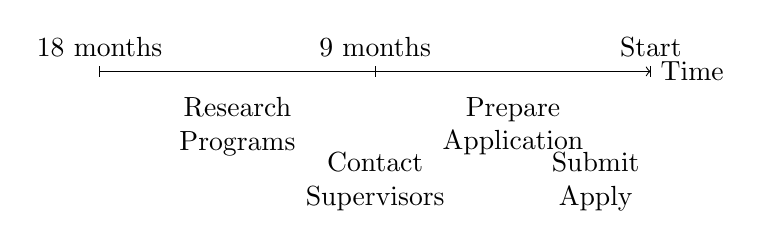
\begin{tikzpicture}[scale=0.7]
    \draw[->] (0,0) -- (10,0) node[right] {Time};
    \draw (0,-0.1) -- (0,0.1) node[above] {18 months};
    \draw (5,-0.1) -- (5,0.1) node[above] {9 months};
    \draw (10,-0.1) -- (10,0.1) node[above] {Start};
    
    \node[align=center] at (2.5,-1) {Research \\ Programs};
    \node[align=center] at (5,-2) {Contact \\ Supervisors};
    \node[align=center] at (7.5,-1) {Prepare \\ Application};
    \node[align=center] at (9,-2) {Submit \\ Apply};
\end{tikzpicture}
\end{frame}

% new page
\begin{frame}[fragile]{Conclusion and Preview of Talk 2}
\begin{columns}[T]
    \begin{column}{0.5\textwidth}
        \alert{Key Takeaways from Talk 1:}
        \begin{itemize}
            \item Diverse PhD structures across Europe
            \item Unique features of German higher education
            \item Strategies for finding opportunities
            \item Importance of tailored applications
        \end{itemize}
    \end{column}
    \begin{column}{0.5\textwidth}
        \alert{Preview of Talk 2:}
        \begin{itemize}
            \item Funding landscape
            \item Financial planning
            \item Practical considerations
            \item Overcoming challenges
            \item Professional development
        \end{itemize}
    \end{column}
\end{columns}

\vspace{0.5cm}
\alert{Detailed Topics for Next Session:}
\begin{itemize}
    \item Comprehensive overview of funding sources
        \begin{itemize}
            \item Government grants, university funding, industry partnerships
        \end{itemize}
    \item Financial aspects of PhD life
        \begin{itemize}
            \item Cost of living, PhD salaries, benefits
        \end{itemize}
    \item Navigating practical challenges
        \begin{itemize}
            \item Work-life balance, cultural adaptation, administrative processes
        \end{itemize}
    \item Building a professional network
    \item Strategies for career development
\end{itemize}

\vspace{0.3cm}
\centering{\textbf{Join us next time for in-depth insights on thriving during your PhD journey!}}
\end{frame}


\end{document}
